\documentclass
[
	12pt,
	a4paper,
	oneside,
%	titlepage
]{article}
%titlepage prints the title on it's own page in article class

%doublespace my text
\renewcommand{\baselinestretch}{1.5}

%reduce the hyphenation of words
\sloppy

%prints a small space between paragraphs and removes the indenting of the first line
\setlength{\parskip}{2ex plus0.5ex minus 0.2ex}
\setlength{\parindent}{0em}

%csquotes - provides multilingual quoting - keeps babel happy
\usepackage{csquotes}
%babel required for biblatex to work. Specifying british last make it the language in use
%\usepackage[english,british]{babel}
\usepackage[british]{babel}

\usepackage[style=authoryear,backend=biber,
	giveninits=true,
	uniquename=init,
	citestyle=authoryear,
	dashed=false,
	maxcitenames=2,
	maxbibnames=99,
	sorting=nyt,
	language=british]{biblatex}

%Add a comma between name and year in citations
\renewcommand*{\nameyeardelim}{\addcomma\space}
%put double space between entries in the references
\setlength\bibitemsep{2\itemsep}

%remove hanging indent from the reference list
\setlength\bibhang{0em}

%Ensure all names in reference list are formatted as Surname, I.
\DeclareNameAlias{default}{last-first}
\DeclareNameAlias{sortname}{last-first}

%Code to format journal article volume and issue as v (i)
\renewbibmacro*{volume+number+eid}{
	\printfield{volume}
	\setunit*{\addnbspace}
	\printfield{number}
	\setunit{\addcomma\space}
	\printfield{eid}
}
\DeclareFieldFormat[article]{number}{\mkbibparens{#1}}

\usepackage{graphicx}

\defbibnote{needsfixing}{\emph{(this formatting needs looking at -- 
	not currently to LSBU standards. )}}
	
% Add my bibliography file here
\addbibresource{references.bib}

%rotating allows text to be printed sideways
%multirow allows tables with cells spanning more than one row
% Remove this if not required
%\usepackage{rotating,multirow}


\begin{document}
\author{Gregory Cartwright}
\title{Does level of frailty influence advance care planning 
	for community hospital inpatients?
}
\maketitle
\begin{abstract}
Community hospital patients generally have multiple co-morbidities and varying
levels of dependence. The prevalence of frailty is therefore likely to be high.
Whilst these patients are usually clinically stable when admitted, their health
can deteriorate. This deterioration can often be addressed in the community hospital
but sometimes for optimal management it is necessary for the patient's treatment to be
escalated to an acute setting. The risks of such transfers for people with frailty are high
and sometimes outweigh the benefits, and outcomes may be better if the transfer
does not happen. This is not always easily appreciated during the out of hours period.
Patients with frailty should be involved in discussions about
potential deterioration and advance care plannning should be undertaken.

This study aims to retrospectively evaluate the care of 100 community hospital
patients to assess if there is an association between level of frailty and advance
care planning and to provide guidance for future practice to 
help avoid unhelpful escalation of treatment and improve patient outcomes and 
experience.
\end{abstract}
\section{Introduction}

The population of the UK is getting older and this trend is forecast to continue.
In 2016 18\% of the population was over 65 years old, with 2.4\% over 85 years old.
Both these figures are expected to grow over the next 20 years \parencite{ons:17}.
Frailty is widely agreed to be a condition where the maintenance of homeostasis 
becomes vulnerable to 
small stressors \parencite{vellas:16}.  Examples of such stressors include changes in environment and minor
illness. The consequences of exposure to these include delirium, significant reduction in mobility,
falls, increased dependency, non-specifc failure to thrive and death 
\parencite{bgs:14,oliver:14,vellas:16}.
The prevalence of frailty amongst the ageing population is high \parencite{clegg:13},
with about 10\% of those aged over 65 and up to 50\% of
those aged over 85\% having frailty \parencite{bgs:14}. These figures
are thought to be higher still in the group of people that are housebound, 
have care at home or live in a care home \parencite{oliver:14}.

The author is an advanced nurse practitioner (ANP) in a community Trust.
The Trust has community hospitals which have wards for inpatient rehabilitation and
medical stepdown. There are 12 wards accross 8 community hospitals. Each ward has
an ANP who works on the ward to provide medical management of the patients during 
the hours of Monday to Friday, 0900 to 1730. Outside of these hours, medical care 
is provided by the out of hours (OOH) general practitioner (GP) service. 

Most patients are admitted to the community hospital wards for either rehabilitation
or medical stepdown. The majority of these patients come following an acute admission
where they have been stabilised medically but are often deconditioned as a result
of acute illness and are not ready to go home. At this stage their needs include 
ongoing medcial treatment and monitoring and further assessments and treament such 
as physiotherapy and occupational therapy to prepare them for discharge home.

Some patients are admitted directly from home because they have medical or rehabilitation
needs that cannot be met at home but don't require an admission to an acute hospital.
A minority of patients are admitted for paliative care.

When patients are admitted to one of these wards they have a comprehensive geriatric 
assessment (CGA) \parencite{bgs:14} performed by the multi-disciplinary team (MDT).
An international meta-analysis found that, when compared with general medical care,
CGA was effective at keeping older people alive and living in their own homes at
twelve months post admission with a number needed to treat of 33 \parencite{ellis:11}.

The author expects that many of the patients admitted to the wards have frailty.
The numbers of patients with frailty is not known, however the patients are assessed 
for frailty and the patients admitted are old. During the last financial year the
average age was 81 and 49\% of patients admitted were aged 85 or over. Many have 
care needs as seen above.

Although the patients are usually clinically stable when they arrive on the ward,
their condition can deteriorate. This is usually managed in the community hospital
ward environment. The patients can have investigations including blood tests, plain
xrays and electrocardiograms (ECG) usually without leaving the community hospital.
They can also recieve treaments such as intravenous (IV) fluids, IV antibiotics
and even blood transfusions. 

Sometimes the deterioration is such that, 
for optimal management, services are required that can only be offered in secondary 
care. When this is the case a decision has to be made, weighing up the proposed
and likely benefits of transferring the patient as an urgent or emergency case to
an acute hospital with the risks that this presents to the patient. During the in-hours
period this decision is made by the ANP who may liaise with the consultant geriatrician. During
the OOH period the nurses make a telephone referral to the OOH GP.

This decision making is difficult for the OOH GP who usually does not know the patient.
Also the patient is acutely unwell and may not be able to participate in discussions
about their care. If it is nighttime it may be difficult to contact relatives to 
have such discussions. In these circumstances it could
be argued that the safest option is to admit the patient to the ED where their 
condition can be further assessed and closely monitored.

There is evidence that patients with frailty often have poor outcomes, including death,
following admission to acute hospital \parencite{silver:12, wallis:15}. 
This is recognised by the ANPs and for some frail patients they 
will have discussions with the patient and their family about the relative risks
and benefits of a potential admission to an acute hospital and what they would want to 
happen in the event of deterioration in their health. This way a person-centered 
advance care plan (ACP) can be made before any deterioration happens.

When patients deteriorate during the OOH period and the patient
gets sent to the acute Trust, the ANP retrospectively reviews what happened to see if the admission
could have been avoided. There are times when the ANP feels that, in those particular
circumstances, the risks to the patient of the acute admission outweigh the benefits
due to their frailty, and that the patient should have had an ACP
to avoid this acute admission. Some partients have an ACP made before admission 
and there are also patients who decline the process of advance care planning, however it appears 
that there are patients for whom an ACP is not considered when it really should be.

The level of frailty of patients is recorded but not formally used to guide advance
care planning. This project aims to examine if there is an association between the 
level frailty in these community hospital inpatients and whether advance care planning
is undertaken.

\section{Literature review}

A literature search was performed using the London South Bank University Library 
online catalogue. The search engines used were CINAHL Complete and MEDLINE. The
search terms used were ``frailty assessment", ``frailty outcomes" and ``frailty 
interventions".

\subsection{Assessing frailty}
An international systematic review found 
that at least 10\% of people aged over 65 had frailty and of those aged 85 or over
at least 26\% were frail \parencite{collard:12}. There are various methods and tools used to assess frailty.
Some of these count the number of deficits from a particular set that a person has. 
\textcite{sternberg:08} suggest that such a tool is not practical for use in a clinical
setting, being more suited to assessing populations for strategic planning. 
Other tools require numerous specific measurements to be taken, again making them
less suitable for clinical use \parencite{martin:08} and possibly more suited to research purposes
\parencite{ensrud:08}. \textcite{romero-ortuno:16} argue that this fragmentation should not
be viewed as a problem as each frailty assessment tool is suited to a different 
purpose. 

In both the clincal area which the author works and the emergency department at
the local acute Trust, frailty is assessed using the Clinical Frailty Scale (CFS).
See appendix~\ref{appendix:CFS}.
The CFS is a tool that has been validated for use in cinical practice 
\parencite{rockwood:05}. It rates frailty based on the person's level of independence
and dependence, giving them an ordinal postion on the continuum from very fit and completely 
independent, CFS of 1, to very severely frail and completely dependent, CFS of 8.
There is also a CFS of 9 for those who are terminally ill. The CFS is based on clinical
judgment of the patient and is therefore suited to clinical use, certainly after
the patient has had a CGA \parencite{bgs:14}.

Generally, the majority of the population of community hospitals is frail older 
people \parencite{silver:12}.
The CFS score has recently been introduced to the community hospital wards in the author's Trust. The
score is not being used for any specific purpose, it is just being entered into 
the patients' notes for people to refer to. These scores are not being collected, 
but the author suspects that the proportion of inpatients who are at least 
moderately frail, with CFS at least 6, will be quite high. Specifically because
CFS is partly based on a person's ability to carry out activities of daily living (ADLs)
and instumental activities of daily living (IADLs) and one reason that many patients
are admitted to the community hospital is that they need rehabilitation to be
able to carry out ADLs and IADLs. Indeed in a study to assess the prevalence of frailty
in France, \textcite{cossec:16} found that dependency on others for IADLs was an 
independent determinant of frailty.

\subsection{Consequences of frailty}

By definition, frailty is a state where a small change, intrinsic or extrinsic, can
lead to multiple consequences \parencite{collard:12}. These can be severe, including 
death. An examination
of all bereavements of adults in England that were not due to accident, homicide or suicide for 
a four month period in 2012 was 
carried out \parencite{ons:13}. It found that the proportion of deaths
that were not due to cancer or any cardiovascular disease (CVD) was 42\%. In the over 80
age group this was 80\%. The most recent edition of this survey from 2015 found
that the overall proportion of non-cancer and non-CVD deaths was slightly higher 
at 46\% \parencite{ons:16}, but did not provide a breakdown by age group. They 
did however report that 60\% of their sample were aged over 80.

How many of these deaths were due to frailty is not know, however 
a Canadian study that examined all deaths in Alberta found that frailty was the
cause of 30\% of mortality \parencite{fassbender:09}.

A national guide for emergency and urgent care of older people \parencite{silver:12}
reports that many older people are admitted to hospital only to die within hours.
This is particularly true for people admitted during the out of hours period.
Whilst this does not quantify the sequelae of frailty, there is literature that 
supports this. \textcite{wallis:15} performed a retrospective study looking 
at outcomes of hosptial admission for people aged 75 and over, in relation to CFS. 
They found that increased frailty was an independent predictor of both 30-day
readmission and in-patient death, with nearly a quarter of people with CFS of 8 dying 
during the admission. This supports the work of \textcite{kang:15} whose Chinese 
study also found that frailty was independtly associated with an increased risk of 
inpatient death, and also significantly increased the risk of readmission and 
3-month mortality for those who survived to hospital discharge.

The effect of frailty on those discharged from hospital was also studied by 
\parencite{kahlon:15}, who also found that frailty significantly increased the 
risk of both readmission and death within 30 days of discharge.

\subsection{Interventions for frailty}
Frailty is clearly a problem, so what should be done about it? Older patients 
should be screened for frailty at every contact with a health professional 
\parencite{bgs:14}, and 
this is already happening in the community hospital wards. There is a consensus that 
frailty should be viewed as a syndrome with multiple domains and therefore
there should be an MDT approach to it's management \parencite{vellas:16}.

The CGA is a multidisciplinary, evidence based strategy to guide the management 
of frailty that is viewed as best practice \parencite{silver:12, bgs:14, oliver:14}. Patients
in the communtity hospitals already recieve this regardless of their CFS score.

We have seen how frailty combined with acute illness carries a high risk of death, and 
\textcite{silver:12} reports that end of life care in older people with frailty
is something that is often not adequately considered. \textcite{oliver:14} support this
by asserting that people with frailty are often not involved in planning their 
end-of-life care. They suggest that the reasons for this include factors such as
the trajectory, with frailty often being a more gradual decline without sudden 
landmark moments. This contrasts with conditions such as terminal cancer where there 
is a defining transition to an end-of-life phase. This can mean that entering such a
phase is not recognised and therefore planning is overlooked. 

Should the recognition of a high level of frail act as an event to signify
that a person is entering an end-of-life phase? Having found that frailty in the 
context of acute coronary syndrome is associated
with poor outcomes, \textcite{kang:15} recommend that a high CFS should
trigger the consideration of escalation pathways \parencite{kang:15}.
This supports the recommendations of \textcite{silver:12} who assert that over-investigation
and uncessary interventions in the frail elderly population are costly to both the
individual and the health economy. They go on to advise that in such patients, 
their preferences for their future care should be ascertained early. \textcite{oliver:14} 
reinforce this by highlighting the importance of gathering this information
before the person loses the capacity to make decisions about how their care should
progress. The later work of \textcite{romero-ortuno:16} adds weight to this argument.
Having identified the increased risk associated with frailty and hospital admission, 
they recommend that frailty generally should trigger personalised planning of
care and it's escalation.

\section{Aim and objectives}

\subsection{Aim}
The overall aim of this study will be to examine if there is a relationship between
level of frailty of community hospital in-patients and whether advance care planning
happens and what other factors might influence this process.

\subsection{Objectives}

\begin{enumerate}
\item	Ascertain the prevalence of different levels of frailty within the local community
		hospital population, and within these levels identify how many do not have
		an ACP before admission.\label{obj:prevalence}
\item	Identify how many of these patients have subsequent consideration of preemetive planning
		of treament escalation during their in-patient stay.\label{obj:association}
\item	Formulate local recommendations for practice to help reduce unhelpful
		acute hospital admissions for people with frailty through more effective
		preemtive planning of treatment escalation.
\end{enumerate}

\section{Study design} 
\label{sec:design}
The objectives require collection of numbers
and proportions of patients that meet objective criteria. A quantitative design
will be appropriate to this approach \parencite{parahoo:14}.

The study aims to examine the association between variables of 
the level of frailty and whether preemtive planning
was carried out. It therefore seems appropriate to use a correlational design. 
It will be a retrospective observational 
cross-sectional study: the casenotes of discharged patients will be reviewed. To achieve 
objective~\ref{obj:prevalence}
data will be obtained by reviewing the case-notes
of patients, examining the initial MDT assessments to ascertain CFS score, 
whether a treament escalation plan was in place prior to admission and other aspects
of the patient and their admission that could be relavent to preemetive escalation
planning. For objective~\ref{obj:association}, the entire case-notes of patients 
will be reviewed to ascertain whether preemetive planning of treament escalation 
was considered during the stay. 

\section{Sample}
Time for data collection is limited due to the timescale for the dissertation. 
Therfore the sampling method needs to capture as many patients as possible in a 
short time. To facilitate this a convenience sampling method will be used.

An electronic patient record (EPR) is currently being rolled out across the Trust.
Currently eight out of the twelve wards have this implemented, so all the patient 
records for patients on these wards are accessible by the author remotely. This
accounts for 148 of the total of 214 beds: 69\%. 

The size of the sample will be 100 patients. To obtain this sample, the first 100
patients discharged from EPR wards on or after 1 December 2017 will be included.
This method allows the full duration of the admission to be studied. The average
length of stay (LOS) is 20.4 days.

\section{Research instrument}

The data collection tool that will be used is 
provided in appendix~\ref{appendix:tool}.

\section{Procedure}
\label{sec:procedure}
For each member of the sample, the EPR will be reviewed. 
For objective \ref{obj:prevalence} 
the initial admission and clerking documentation will be reviewed to obtain
record the CFS score and the other relevant data. This will be recorded in the tool.


To collect data for objective \ref{obj:association}, all patients who do not have
a pre-existing plan will then have their EPR searched
for the duration of their admission. The record will be searched for the following
terms:

\begin{itemize}
\item acute
\item escalation
\item advanced care plan
\item deterioration
\end{itemize}

Where one of these terms is found, the record will be read in context to assess if 
escalation planning was being considered. If preemtive planning of treatment escalation
was considered at least once during the admission then this will be recorded as ``YES"
in the data collection tool. Otherwise ``NO" will be recorded in that collumn.

\section{Data analysis}
\emph{I need some help from my supervisor with this section}

\section{Ethical considerations}

This proposal will be submitted to the research department at the Trust to gain 
their approval for the study to be conducted. The result of this correspondence 
will be included in this document as an appendix.

\textcite{biggam:15} identifies five ethical principles that research should maintain:
\begin{enumerate}
\item Do no harm
\item Impartial
\item Transparent
\item Confidential
\item Voluntary
\end{enumerate}

\subsection{Do no harm}
This study will not influence the care or treament of any current patients therefore
there is no possibility of it causing harm to patients.

\subsection{Transparent}
This document sets out clearly how the study will be conducted.

\subsection{Impartial}
The author is an employee of the Trust where the study will take place. If any bad
practice is discovered as part of the work undertaken then the relevant manager
will be informed. It is not expected that the author is a relative of any of the patients
whose notes will be examined as part of the study. If it transpires that such a 
relationship exists then that patient will be excluded from the study to eliminate
any possiblity of bias.

\subsection{Confidential}
To ensure that the confidentiality of patients is maintained during this study there
will be no recording of patient identifying data outside of the EPR. Each patient
record will be allocated a study ID number which will be recorded in the data collection
tool, see appendix~\ref{appendix:tool}. This will anonymise the records.

The data collection tool will be an electronic Microsoft Excel 2010 spreadsheet
which will be stored on a Trust owned laptop which is encrypted and password protected. A backup 
of the data will be maintained on a secure Trust server which will be accessed over
the secure Trust network. All the data will be destroyed one year following completion 
of the study; May 2019.

\subsection{Voluntary}

This project looks at retrospective data following patient discharge to evaluate 
an aspect of patient management. As such, this criteria is not relevant.

\section{Timetable}
Here is the proposed timtable for completion of this dissertation:
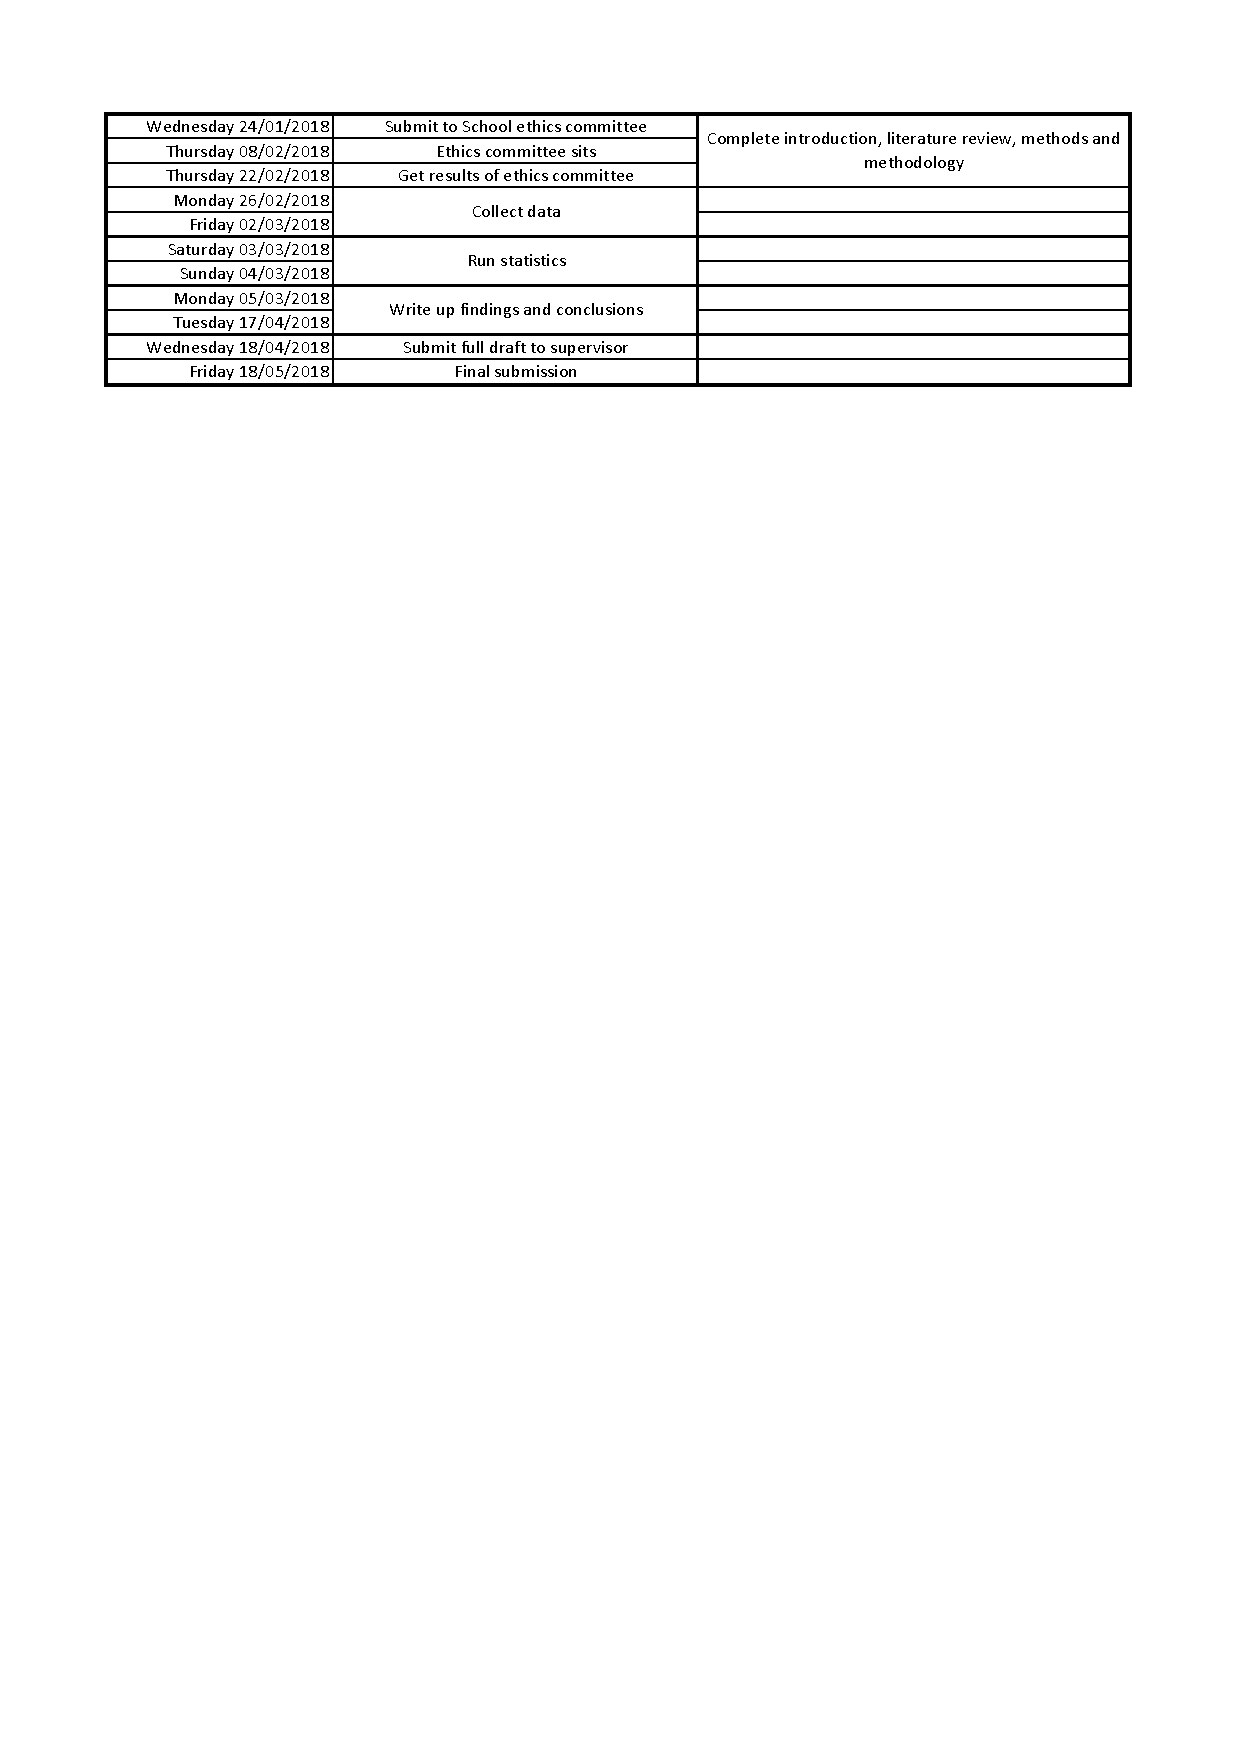
\includegraphics[width=\textwidth]{DissertationSchedule}

\section{Planned style of dissertation}
A traditional style of dissertation is planned.

\clearpage
\printbibliography[prenote=needsfixing]

\clearpage
\begin{appendix}

\section{Clinical Frailty Scale}
\label{appendix:CFS}
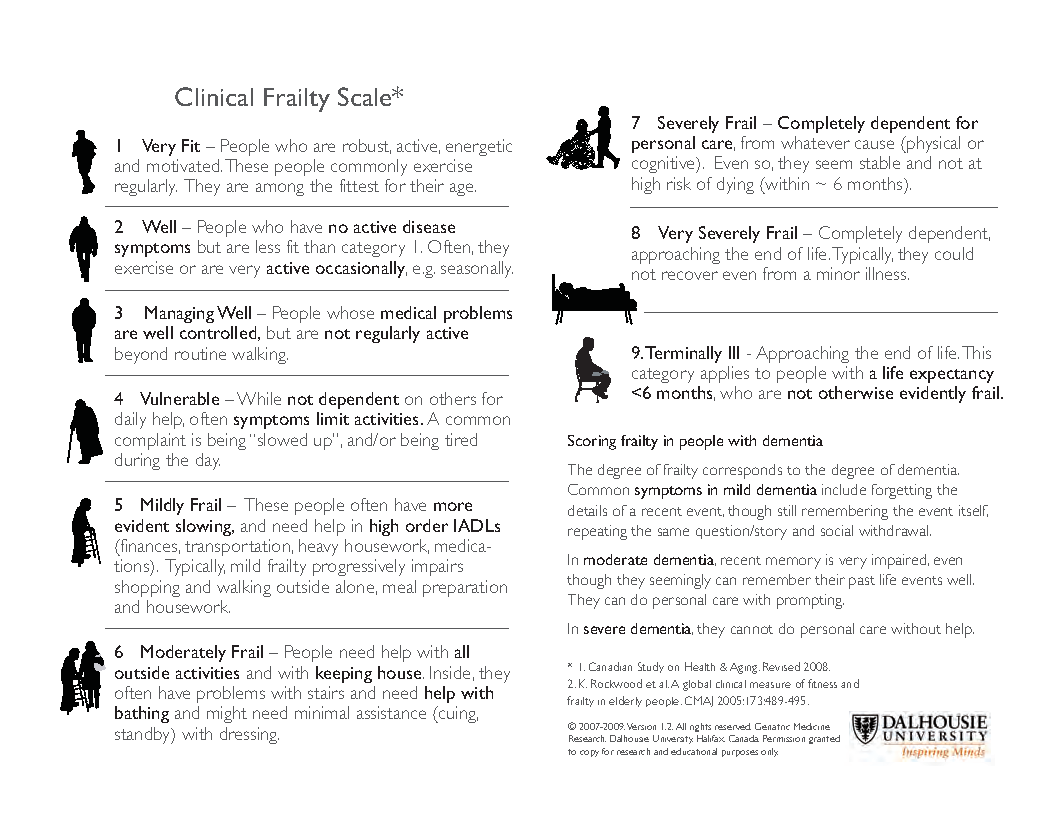
\includegraphics[width=\textwidth]{CFS}

\section{Data collection tool}
\label{appendix:tool}
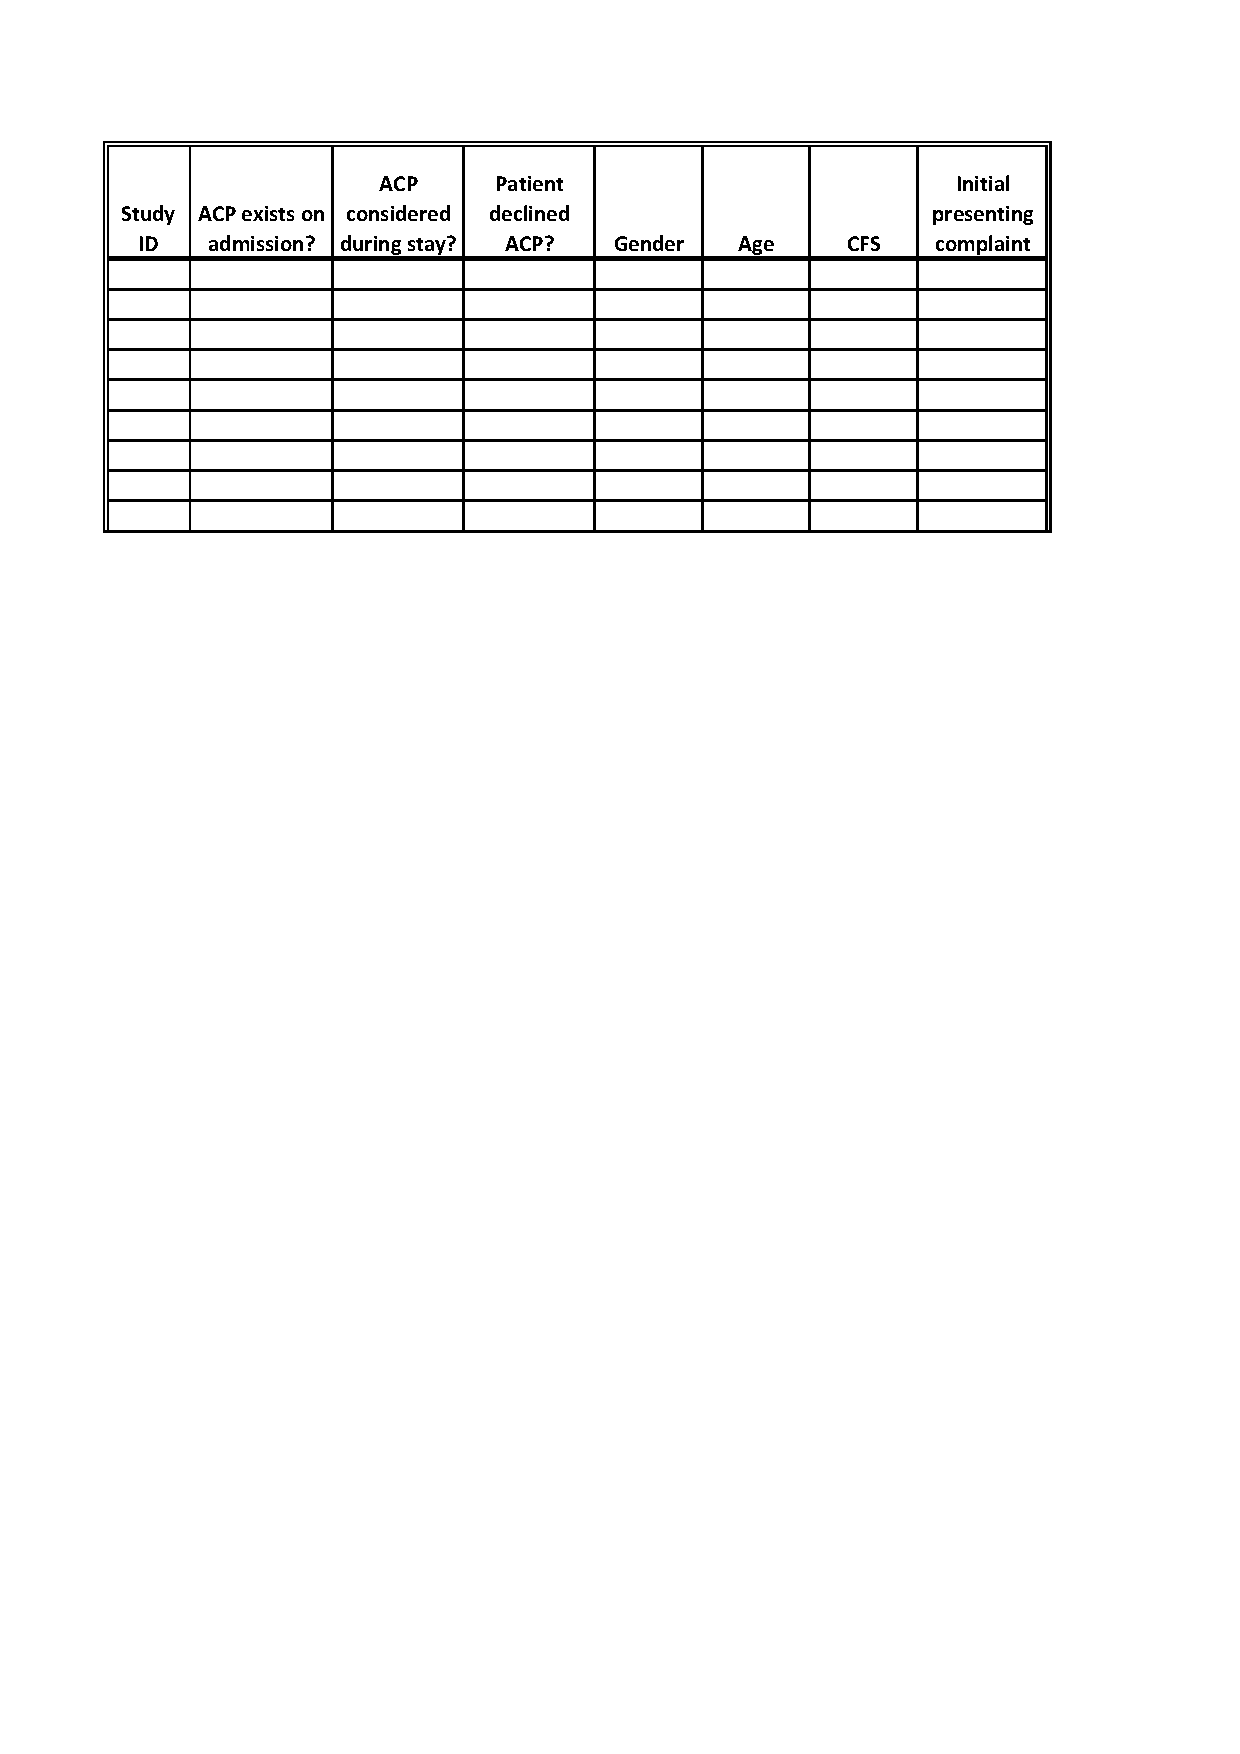
\includegraphics[width=\textwidth]{dataCollection}
\end{appendix}

\end{document}
